%!TEX root=gm_jmlr.tex
In this section, we analyze Gradient Boosted Regression Trees (GBRT) in detail and give insights of unique properties of GBRT. We compare GBRT with a linear classifier and a kernel classifier. Let $\theta$ denote the parameters of a classifier $H$. The goal of learning a classifier is to learn these parameters $\theta$ by minimizing a loss function $\ell$. These parameters are usually learned by gradient descent, where at each iteration, we compute the gradient of the loss function $\ell$ w.r.t. parameters, $\frac{\partial \ell}{\partial \theta}$. We apply the generalized chain rule, and decompose this gradient into two parts:
\begin{align}
	\frac{\partial \ell}{\partial \theta} = \sum_{i=1}^n \frac{\partial \ell}{\partial H(\x_i)} \frac{\partial H(\x_i)}{\partial \theta}, \label{eq:chainrule}
\end{align}  
where $H(\x_i)$ is the prediction of input $\x_i$. Note that the first part $\frac{\partial \ell}{\partial H(\x_i)}$ is the gradient of the loss function $\ell$ w.r.t. predicting function in the function space evaluated at an input $\x_i$, and the second part is the gradient of the predicting function w.r.t. its parameter $\theta$. Compared to linear classifiers and kernel classifiers, there are two unique properties of GBRT: implicit parameterization and non-linear feature combination.

\subsection{Implicit parameterization} Both linear classifier and kernel classifier have a predicting function $H$ that can be represented as an analytical function of its parameters (\emph{i.e.} for linear classifier, $H(\x) = \x^\top\theta$, where $\theta \in {\cal R}^p$). Therefore, when optimizing a linear or a kernel classifier, one usually optimizes the classifier parameters directly through the gradient of the loss w.r.t. classifier parameters (\emph{i.e. }$\frac{\partial \ell}{\partial \theta}$). In contrast, there is no such an \emph{analytical} function to model the predicting function $H$ in GBRT, and one has to learn the parameters of the GBRT predicting function in two steps. In other words, GBRT is parameterized implicitly. First, GBRT computes the gradient of the loss function w.r.t. the predicting function $H$ in function space $\frac{\partial \ell}{\partial H(\x_i)}$ evaluated at each input sample $\x_i$. Second, GBRT approximates this functional gradient $\frac{\partial \ell}{\partial H(\x_i)}$ at every input $\x_i$ by building a limited depth regression tree $h(\cdot)$ using the CART algorithm, which minimizes a squared impurity function (\ref{eq:CART}). Note that features are only used when approximating the negative gradient during the second step, and therefore we can add constraints for feature extraction here. This two-step optimization procedure provides more flexibility to incorporate structured feature information commonly used in bio-informatics and computer vision. However, these two steps are also very closely connected, and we will show their connections in Section~\ref{sec:greedymiser}. 

\subsection{Nonlinear feature combination} Different from linear classifiers, GBRT is capable of approximating a non-linear gradient surface. Figure~\ref{fig:simul} (plot (a)), shows a scenario where sample inputs are not linearly-separable. Plots (b)-(d) show the functional gradient surface $\frac{\partial \ell}{\partial H}$ of each classifier. GBRT approximates the gradient surface through limited depth regression trees. For a depth $3$ tree, which has $2^{3-1} = 4$ leaf nodes, GBRT essentially approximates the gradient surface by partitioning the space into 4 blocks (shown in plot (d)). In contrast, a linear gradient is just a hyperplane in the input space (\emph{i.e. } $\x^\top (\frac{\partial \ell}{\partial \theta})$), which is shown in plot (b). Kernel classifiers can achieve non-linear gradients through the kernel-trick, shown in plot (c). However, the key advantage of GBRT is that it achieves this non-linearity in a parametric way. For a depth $3$ tree, its parameters are only $3$ features and corresponding splitting values. In contrast, kernel methods achieves non-linearity through a non-parametric kernel that depend on the size of the data. During test-time, parametric GBRT is much faster than non-parametric methods and therefore is very suitable for large scale data sets and test-time cost-sensitive applications. 
 
\begin{figure*}[t!!!]
\centerline{
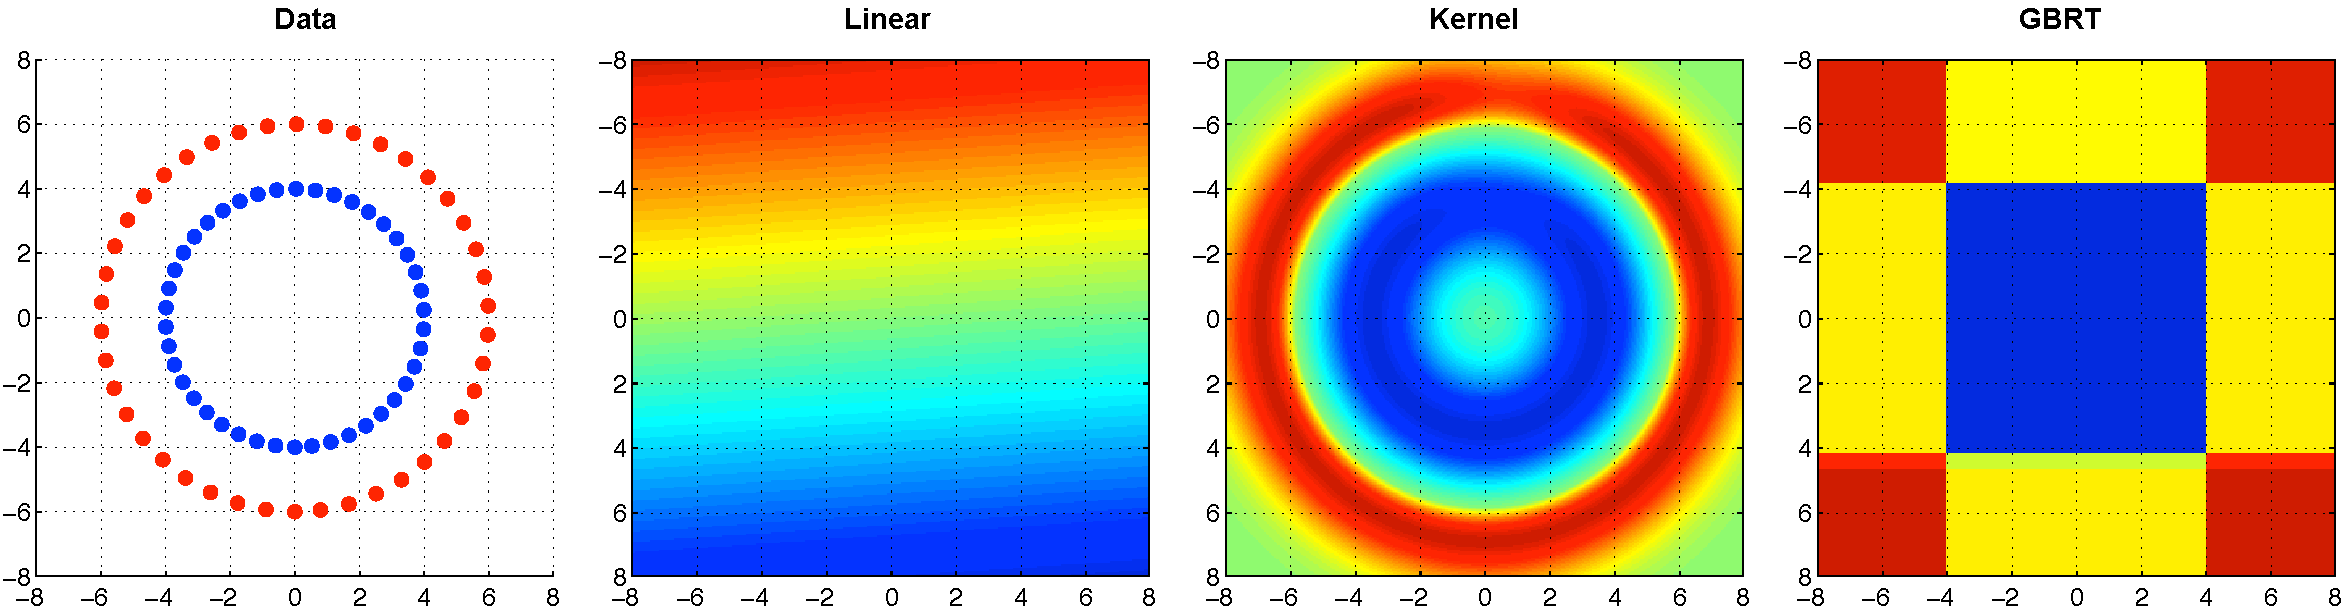
\includegraphics[width = \textwidth]{plots/grad_simul.pdf}%{plots/simul_iter}
}
\caption{Gradient surface of linear, kernel and GBRT classifiers. (a) The linearly-unseparable simulation data. Red dots and blue dots are from two different classes, and the task is binary classification. (b) The gradient surface of a linear classifier, which is a hyperplane (c) The gradient surface of a kernel classifier. Kernel methods achieve non-linear gradient surfaces in a non-parametric way. (d) The gradient surface of a GBRT classifier. }
\label{fig:simul}
\end{figure*}





% \textbf{Implicit parameterization.}
% However, the first key difference between GBRT and classifiers that are commonly combined with manifold regularization (e.g., linear and kernelized logistic regression, support vector machines, least squares regression) is that the predicting function $H(\cdot)$ of GBRT \emph{is not explicitly parameterized}. Specifically, $H(\cdot)$ is not an analytical function of its parameters
%  (i.e. decision tree splitting features and corresponding splitting values). Therefore, we cannot compute the gradient $\frac{\partial H(\x_i)}{\partial \theta}$. In contrast, the majority of other classifiers have predicting functions that can be represented as an analytic function of its parameters,
%  and the gradient in eq.~(\ref{eq:chain_gradient}) can be computed normally. Without an explicit parameterization for $H(\cdot)$, gradient boosting requires a function to approximately match the functional gradient $g(\cdot) = \frac{\partial {\cal L}}{\partial H(\cdot)}$ \emph{directly}.
%
%
% \textbf{Discontinuous gradient approximation.}
% GBRT approximates the functional gradient $g(\x)$ at every input $\x$ using a limited depth regression tree $h(\x)$, as shown in eq.~(\ref{eq:cart}). Note that a depth $d$ tree makes at most $2^{d-1}$ different predictions. Therefore, this approximation is discontinuous wherever the regression tree splits on a feature. Because this approximation is done using regression trees, \emph{the similarity of functional gradients for nearby inputs is not guaranteed}. We demonstrate this difficulty on a synthetic binary classification dataset.
%
% Figure~\ref{fig:illu} depicts a simple one-dimensional dataset with two known labels. We plot the predictions passed through link function $\sigma(\cdot)$ that we obtained from GBRT with manifold regularization after different numbers of iterations. In each plot, the vertical black lines indicate the regression tree at the current iteration split the data. We initialize the predicting function to be $H^0(\x_i) = H^0(\bar{\x}_j) = 0; \forall i,j$ (as we have no prior for the labels of unlabeled inputs), and thus all inputs have link value $\sigma(H^0(\x)) = 0.5$. At the first iteration, because all inputs have the same prediction, only labeled inputs (the first and last) have non-zero gradient (from the loss $\ell(\cdot)$). Thus, GBRT learns a regression tree to predict the first input closer to 1 and the last input closer to 0, while keeping the predictions of unlabeled inputs unchanged. The second iteration again only the predictions of the first and last inputs change. At the fifth iteration the dataset is still largely unchanged save a few inputs neighboring the first and last inputs. Even after 100 iterations roughly one third of the dataset has predictions identical to their initial predictions. Finally, after 500 iterations the dataset is clearly separated. In effect, GBRT with manifold regularization will require a large number of trees, even for simple datasets, to propagate gradients of labeled inputs to nearby unlabeled inputs. We refer to this problem as  \emph{gradient propagation delay}.
%





